\chapter{Theoretische Grundlagen}

\section{Aerodynamische Wirkweise des Rotors}
In der Welt der Windenergieerzeugung gibt es zwei grundlegende Bauformen von Windkraftanlagen: die Horizontalachsenwindkraftanlagen (HAWTs) und die Vertikalachsenwindkraftanlagen (VAWTs). Während Vertikalachsenanlagen bestimmte Vorteile in Bezug auf die Windrichtungsunabhängigkeit und die einfache Wartung aufweisen, haben sich Horizontalachsenwindkraftanlagen als die effizientere und weit verbreitete Option erwiesen. Diese Effizienz rührt von ihrer Fähigkeit her, höhere Energiemengen aus dem Wind zu extrahieren, insbesondere bei starken und konstanten Windverhältnissen, wie sie häufig in Offshore-Umgebungen vorkommen. Aufgrund dieser Überlegenheit in Bezug auf die Energieausbeute und die technologische Reife konzentriert sich diese Arbeit ausschließlich auf die Betrachtung und Analyse von Horizontalachsenwindkraftanlagen.

\begin{figure}[htbp] % Positionierungsoptionen: h=here, t=top, b=bottom, p=page of floats
    \centering % Zentriert das Bild
    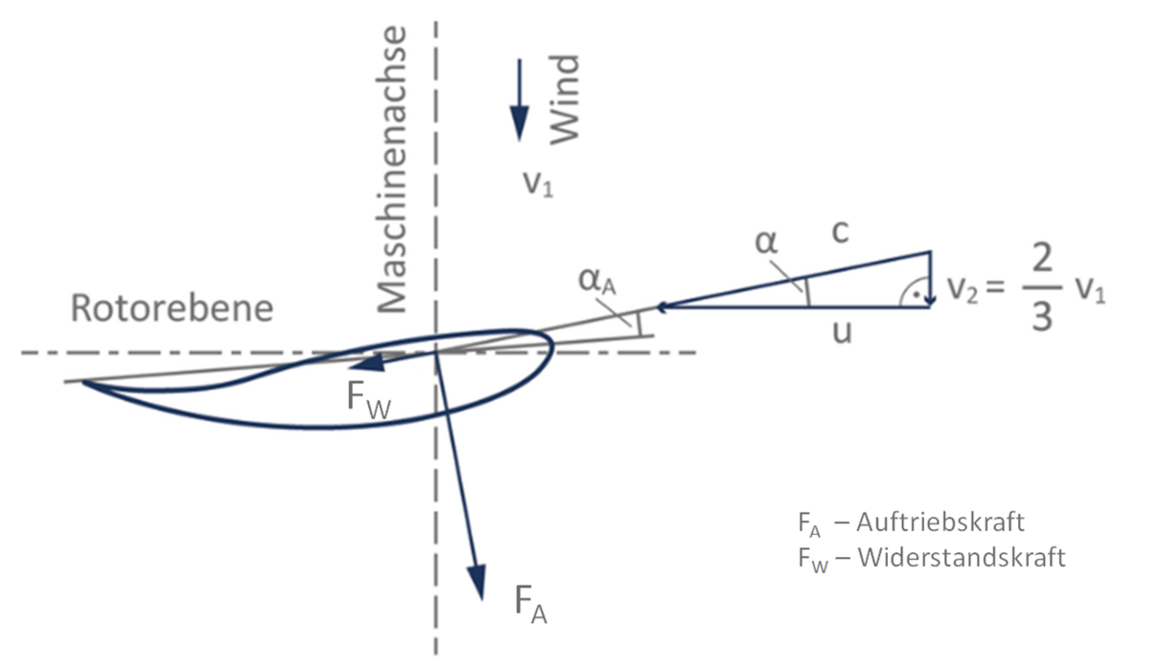
\includegraphics[width=0.8\textwidth]{figures/winddreieck.png} % Pfad zum Bild und Skalierung
    \caption{Kräfte am Rotorblatt resultieren in Drehmoment \cite{noauthor_aerodynamik_nodate}} % Bildunterschrift
    \label{fig:winddreieck} % Label für Referenzen im Text
\end{figure}

Das zugrundeliegende physikalische Prinzip von HAWTs ist das gleiche wie bei Flugzeugflügeln: der Auftrieb.
Der Rotorblattquerschnitt ist so geformt, dass eine Differenz im Luftdruck zwischen der oberen und der unteren Seite des Rotorblattes entsteht, wenn Wind darüber strömt.
Die Unterseite des Rotorblattes erfährt einen höheren Druck als die Oberseite, was zu einer Auftriebskraft führt, die das Rotorblatt nach oben bzw. in Drehrichtung des Rotors zieht.
Die Kraftkomponente des Auftriebs in die Drehrichtung erzeugt um die Drehachse des Rotors ein Drehmoment. Der Rotor dreht sich und treibt den Generator an. Eine Veranschaulichung der Kräfte an einem Schnitt durch das Rotorblatt zeigt \cref{fig:winddreieck}.

\section{Kennzahlen}
Im Folgenden Abschnitt werden die für das Verständnis dieser Arbeit wichtigsten Kennzahlen für den Betrieb eines Rotors kurz erläutert. Für weitergehende Informationen sei auf \textcite{hau_physikalische_2016} verwiesen.
\subsection{Leistungsbeiwert von Windkraftrotoren}
Der Leistungsbeiwert \( C_P \) ist in der Aerodynamik von Horizontalachsenwindkraftanlagen (HAWAs) essentiell und quantifiziert das Verhältnis der nutzbaren mechanischen Leistung \( P \) einer Windturbine zur kinetischen Leistung des Windes \( P_{\text{wind}} \) im Rotorquerschnitt. Die Formel für \( C_P \) ist gegeben durch:

\begin{equation}
C_P = \frac{P}{\frac{1}{2} \rho A v^3}
\end{equation}

wobei \( \rho \) die Luftdichte, \( A \) die Querschnittsfläche des Rotors und \( v \) die Windgeschwindigkeit darstellt. Der Betzsche Grenzwert setzt die theoretische Obergrenze für \( C_P \) auf maximal 59,3\% fest, ausgedrückt als \( C_{P, \text{max}} = \frac{16}{27} \). Dieser Grenzwert basiert auf der Annahme, dass der Wind hinter der Turbine eine Restgeschwindigkeit behält. Real existierende Verlustquellen wie Profil- und induzierte Verluste beeinflussen die Effizienz des Rotors. Moderne Turbinendesigns zielen darauf ab, diese Verluste durch optimierte Rotorblattgeometrie zu minimieren, wobei CFD und BEM-Theorien eine entscheidende Rolle spielen.

\subsection{Schubbeiwert von Windkraftrotoren}
Der Schubbeiwert \( C_T \) ist eine weitere wichtige aerodynamische Kenngröße für Windkraftrotoren, die das Verhältnis der Schubkraft \( F_T \), die durch die Rotorblätter auf den Wind ausgeübt wird, zur kinetischen Energie des Windes im Rotorquerschnitt darstellt. Mathematisch lässt sich \( C_T \) definieren als:

\begin{equation}
C_T = \frac{F_T}{\frac{1}{2} \rho A v^2}
\end{equation}

wobei \( F_T \) die Schubkraft ist. Ein hoher Schubbeiwert kann auf eine effektive Energieübertragung hinweisen, führt jedoch auch zu erhöhten mechanischen Belastungen der Turbinenstruktur. Die Auslegung zielt daher auf ein optimales Gleichgewicht zwischen Energieextraktion und struktureller Belastung ab. Im Kontext der Multirotor-Winkraftanlagen kommt dem Schubbeiwert eine weitere Bedeutung zu. Kontrollierte Schubkraftunterschiede zwischen den einzelnen Rotoren könnten für die Ausrichtung der gesamten Anlage entsprechend der Windrichtung genutzt werden. 

\subsection{Schnellaufzahl}
Die Schnellaufzahl \( \lambda \) oder auch \( TSR \) für Tip Speed Ratio ist ein maßgeblicher Parameter in der Aerodynamik von Windenergieanlagen. Sie berechnet sich aus dem Verhältnis der Umfangsgeschwindigkeit der Rotorblattspitze \( u \) zur Windgeschwindigkeit \( v \) an der Turbine:

\begin{equation}
\lambda = \frac{u}{v}
\end{equation}

Sowohl Leistungs- als auch Schubbeiwert des Rotors hängen von der Schnelllaufzahl ab. Exemplarisch ist eine solche Abhängigkeit in \cref{fig:leistung_vs_TSR} dargestellt. Im Betrieb sollte die Drehzahl des Rotors so geregelt werden, dass die optimale Schnelllaufzahl für maximalen Leistungsbeiwert erreicht wird. Der genaue Wert der Optimalen Schnelllauf hängt vor Allem von der Anzahl der Rotorblätter und deren Design ab. Im Entwurfsprozess werden die Rotorblätter auf eine bestimmte Entwurfsschnelllaufzahl hin optimiert.

\begin{figure}[htbp] % Positionierungsoptionen: h=here, t=top, b=bottom, p=page of floats
    \centering % Zentriert das Bild
    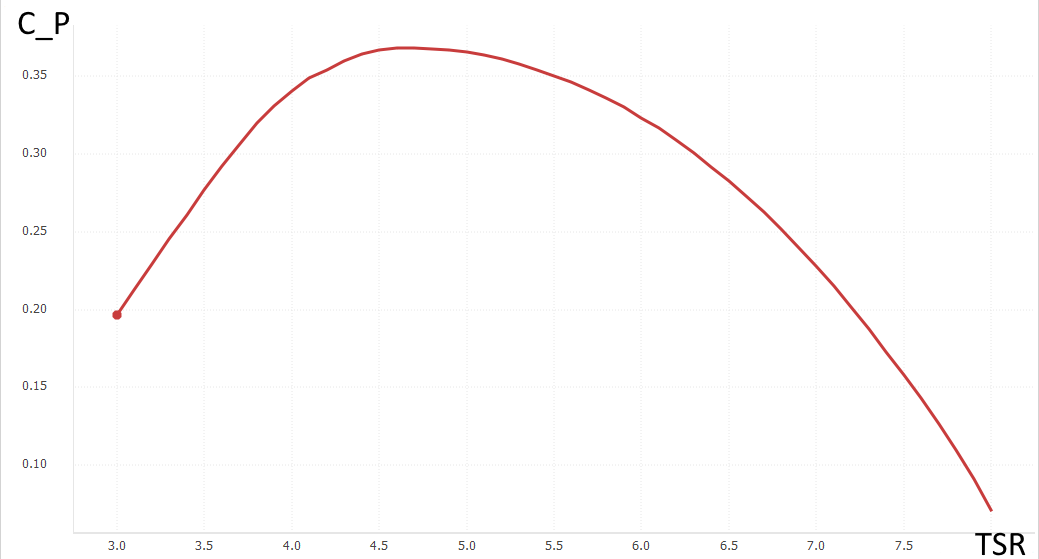
\includegraphics[width=0.8\textwidth]{figures/leistung_vs_TSR.png} % Pfad zum Bild und Skalierung
    \caption{Exemplarische Darstellung des Leistungsbeiwertes \( C_P\) in Abhängigkeit der Schnelllaufzahl \(TSR\) bzw. \( \lambda\), eigene Darstellung} % Bildunterschrift
    \label{fig:leistung_vs_TSR} % Label für Referenzen im Text
\end{figure}

\section{Aerodynamik eines Rotorblattes}
In diesem Abschnitt sollen die wichtigsten Grundlagen der Aerodynamik kurz angesprochen werden. Dabei geht es nur um die Begriffe, die für das Verständnis dieser Arbeit notwendig sind. Ausführlichere Informationen liefert zum Beispiel \textcite{anderson_fundamentals_2017}. 
\subsection{Grundbegriffe eines Profils}
Aerodynamische Profile unterliegen Konventionen zur Beschreibung ihrer Formgebung. Die wichtigsten Begrifflichkeiten werden in \cref{fig:profil_begriffe} dargestellt.

\begin{figure}[htbp] % Positionierungsoptionen: h=here, t=top, b=bottom, p=page of floats
    \centering % Zentriert das Bild
    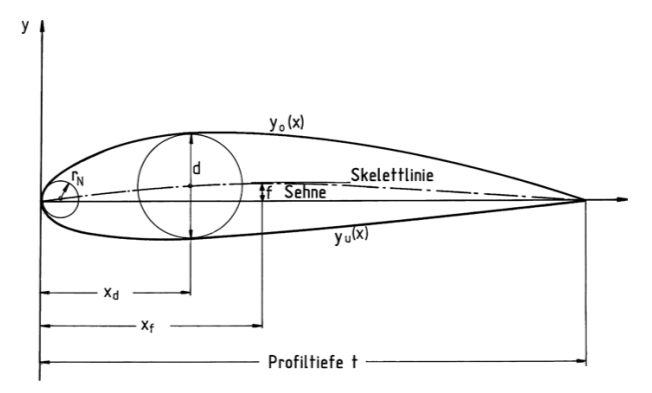
\includegraphics[width=0.8\textwidth]{figures/profil_begriffe.png} % Pfad zum Bild und Skalierung
    \caption{Grundbegriffe bei aerodynamischen Profilen \cite{hau_physikalische_2016}, S.130, modifiziert} % Bildunterschrift
    \label{fig:profil_begriffe} % Label für Referenzen im Text
\end{figure}

\begin{itemize}
    \item Profiltiefe \( c \) (Länge der Sehne)
    \item Maximale Wölbung \( f \)
    \item Wölbungsrücklage \( x_f \)
    \item Maximale Profildicke \( d \), als Durchmesser des größten Kreises auf der Skelettlinie
    \item Dickenrücklage \( x_d \)
    \item Nasenradius \( r_N \)
    \item Profilkoordinaten \( y_o(x) \) und \( y_u(x) \) der Ober- bzw. Unterseite
\end{itemize}

\subsection{Kräfte und Kennzahlen eines Profils}

In der Aerodynamik, insbesondere bei der Betrachtung von Windkraftrotorblättern, sind die Auftriebs- und Widerstandskräfte zentral. Diese Kräfte werden jedoch nicht direkt verwendet, sondern durch dimensionslose Beiwerte dargestellt. Der Grund dafür liegt in der universellen Anwendbarkeit und Vergleichbarkeit dieser Beiwerte.

Der Auftriebsbeiwert \( c_l \) und der Widerstandsbeiwert \( c_d \) ermöglichen es, die Leistung eines Profils unabhängig von seiner Größe oder den spezifischen Flugbedingungen zu bewerten. Der Auftriebsbeiwert \( c_l \) ist definiert als:

\begin{equation}
c_l = \frac{L}{\frac{1}{2} \rho v^2 c}
\end{equation}

wobei \( L \) die Auftriebskraft, \( \rho \) die Luftdichte, \( v \) die Strömungsgeschwindigkeit und \( c \) die Sehnenlänge des Profils ist. Der Widerstandsbeiwert \( c_d \) wird ähnlich berechnet:

\begin{equation}
c_d = \frac{D}{\frac{1}{2} \rho v^2 c}
\end{equation}

Eine Veranschaulichung dieser Kräfte ist in \cref{fig:winddreieck} und \cref{fig:kraft_an_blatt} zu sehen. Dabei ist zu beachten, dass sich die Kräftewirkungen immer auf den aerodynamischen Anstellwinkel des Profils, und nicht auf die allgemeine Windrichtung beziehen. Die Auftriebskraft steht senkrecht zur Anströmrichtung, die Widerstandskraft wirkt in Anströmrichtung. 

Die Gleitzahl, die die aerodynamische Effizienz des Profils angibt, wird als das Verhältnis von Auftrieb- zu Widerstandsbeiwert definiert:

\begin{equation}
E = \frac{c_l}{c_d}
\end{equation}

Dieser Wert gilt nicht für alle Anstellwinkel des Profils. Die Gleitzahl bezieht sich i.d.R auf den Anströmwinkel, bei dem der höchste Wert erreicht wird.
Eine hohe Gleitzahl bedeutet, dass das Profil effizient Auftrieb erzeugt, während der Widerstand gering bleibt. 
Bei Windkraftrotoren ist eine hohe Gleitzahl wichtig, da sie direkt die Menge an nutzbarer Energie beeinflusst, die aus dem Wind extrahiert werden kann. Die Optimierung des Profils zielt daher im Allgemeinen darauf ab, eine möglichst hohe Gleitzahl zu erreichen, um die Effizienz und Leistung der Windturbine zu maximieren.

\section{Grundbegriffe und Geometrie des Rotorblattes}

Schub, Tangentialkraft

\begin{figure}[htbp] % Positionierungsoptionen: h=here, t=top, b=bottom, p=page of floats
    \centering % Zentriert das Bild
    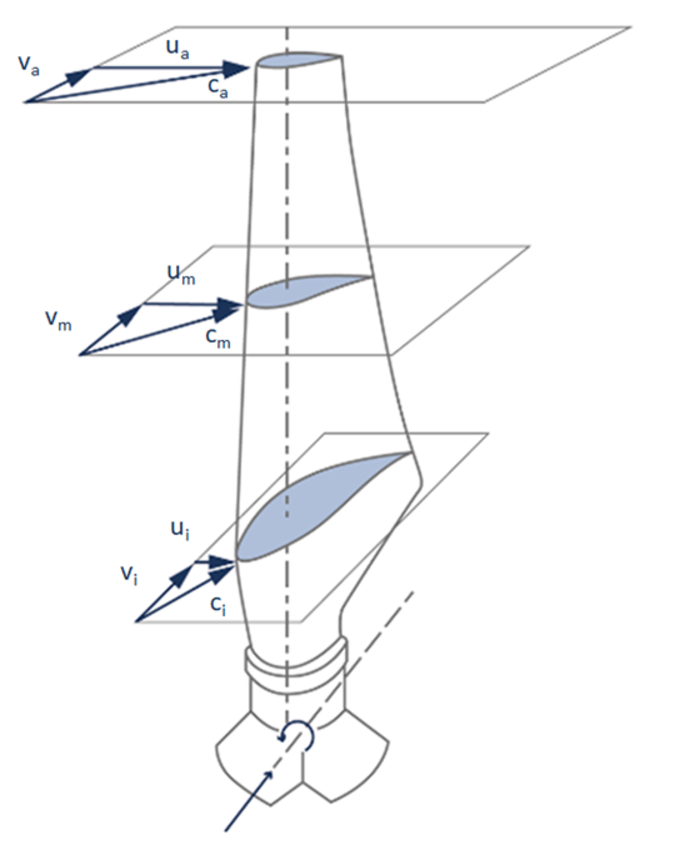
\includegraphics[width=0.8\textwidth]{figures/verwindung.png} % Pfad zum Bild und Skalierung
    \caption{Unterschiedliche Anströmbedingungen entlang des Rotorblattes \cite{noauthor_aerodynamik_nodate}} % Bildunterschrift
    \label{fig:verwindung} % Label für Referenzen im Text
\end{figure}

\begin{figure}[htbp] % Positionierungsoptionen: h=here, t=top, b=bottom, p=page of floats
    \centering % Zentriert das Bild
    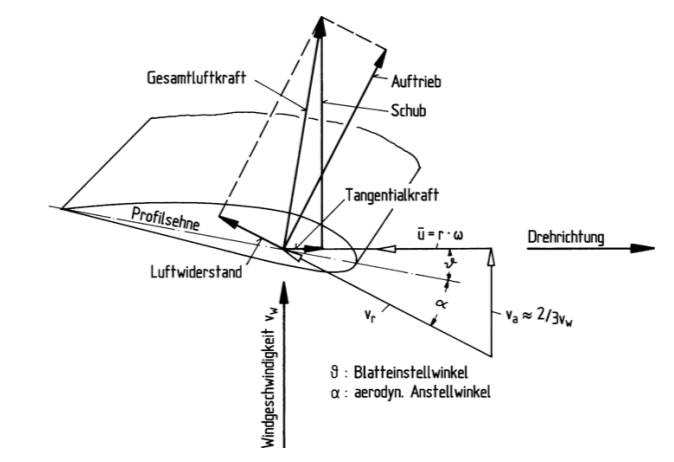
\includegraphics[width=0.8\textwidth]{figures/kraft_an_blatt.png} % Pfad zum Bild und Skalierung
    \caption{Konventionelle Winkelunterscheidung \cite{hau_physikalische_2016}} % Bildunterschrift
    \label{fig:kraft_an_blatt} % Label für Referenzen im Text
\end{figure}

\section{Methoden der Rotorblattauslegung}
\subsection{Auslegung nach Betz und Schmitz}
\label{subsec:betz-schmitz-auslegung}
Die am weitesten verbreitete Theorie der praktischen Rotorblattauslegung basiert auf den grundlegenden Arbeiten von Betz und Schmitz, die Anfang des 20. Jahrhunderts die Grenzen und Möglichkeiten der Windenergienutzung untersuchten. Betz legte mit seinen Theorien den Grundstein und lieferte Beziehungen für die optimale Flügeltiefenverteilung \( c(r) \) sowie die Blattverwindung \( \vartheta(r) \).Seine Theorie geht allerdings davon aus, dass sich die Lustströmung nach dem Rotor lediglich verlangsamt, aber nicht in seiner Richtung abgelenkt wird. Verluste durch den induzierten Widerstand bzw. Blattspitzenverluste sowie Profilwiderstand und Drallverluste vernachlässigt er. Schmitz erweiterte später diese Theorie, indem er zusätzliche Verluste in Betracht zog und so die Auslegung von Rotorblättern weiter verfeinerte.

Die optimale Flügeltiefe  und die Verwindung  eines Rotorblattes lässt sich nach der Theorie von Schmitz aus den folgenden Formeln ableiten: 
\newline

\begin{equation}
c_{\text{opt,Schmitz}} = \frac{16 \pi}{z \cdot c_A} \cdot r \cdot \sin^2 \left( \frac{1}{3} \arctan \left( \frac{1}{\lambda_A }\frac{R}{r} \right) \right)
\end{equation}
\newline

\begin{equation}
\vartheta_{\text{opt,Schmitz}}(r) = \frac{2}{3} \arctan \left( \frac{1}{\lambda_A} \frac{R}{r} \right) - \alpha \left( \varepsilon_{\text{max}}, r \right)
\end{equation}
\newline

wobei \( r \) der lokale Radius entlang der Rotorblattspannweite ist, \( z \) die Anzahl der Rotorblätter, \( C_A \) der Auftriebsbeiwert, \( \lambda_A \) die Auslegungsschnelllaufzahl und \( \alpha \) der Anstellwinkel. \( C_A \) und \( \alpha \) entsprechen sinnvollerweise dem optimalen Betriebszustand der verwendeten aerodynamischen Profile. Die Auslegungsschnelllaufzahl \( \lambda_A \) ist ein frei wählbarer Designparameter. Er kann entweder auf Basis von Erfahrungswerten festgelegt, oder für den betreffenden Anwendungsfall optimiert werden.

Die vorgestellten Formeln bilden die Grundlage für die iterative Entwicklung und das Design von Rotorblättern. Um das so entstandene Design näher zu untersuchen und zu validieren, können Computergestützte Simulationen oder Windkanalversuche durchgeführt werden. Die am weitesten verbreitete Berechnungsmethode wird im folgenden Abschnitt vorgestellt.

\subsection{Simulation mittels diskreter Blattelemente}
Die Aufteilung der Rotorblätter in einzelne Elemente ermöglicht eine wenig rechenintensive Bestimmung der relevanten Kennzahlen. Anders als bei bei der Verwendung von CFD Simulationen können damit ganze Rotoren innerhalb weniger Sekunden berechnet werden.
Die dabei verwendeten Theorien bauen auf einander auf und werden häufig zusammen als BEM-Methode bezeichnet.

\subsubsection{Blatt Element Methode}
Die Blatt Element Methode teilt die Rotorblätter in mehrere kleine Elemente entlang der Spannweite auf und ermöglicht so die Berechnung von Kräften und Momenten auf jedem Abschnitt.
Die Methode basiert auf der Annahme, dass jedes Blattelement die Strömung zwei-dimensional und unabhängig von den anderen Elementen erlebt. Die lokalen Strömungsbedingungen werden durch die Geometrie und die Betriebsbedingungen des Rotors bestimmt. \cite{branlard_wind_2017}
Dies ermöglicht die Verwendung von zweidimensionalen Auftriebs-, Widerstands- und Momentenkoeffizienten zusammen mit der relativen Strömungsgeschwindigkeit, um die Kräfte auf das betreffende Blattelement zu bestimmen.
Die Kräfte werden dann entlang der Spannweite des Blattes integriert, um den Gesamtschub und das Drehmoment zu bestimmen, das durch den Rotor erzeugt wird.

\subsubsection{Blatt Element Momentum}
Die Blatt Element Momentum Theorie erweitert die grundlegende Blatt Element Methode, indem sie Impulserhaltungsprinzipien einbezieht, um eine ganzheitliche Betrachtung der Strömungsverhältnisse am Rotor zu ermöglichen. Während die Blatt Element Methode sich auf die lokale Analyse der aerodynamischen Kräfte an diskreten Blattelementen konzentriert, integriert die BEM-Theorie diese lokale Betrachtung mit der globalen Wirkung des Rotors auf den Luftstrom auf Basis der Impulstheorie.\cite{branlard_wind_2017}
Um die Genauigkeit der Vorhersagen weiter zu steigern, werden in einigen Formulierungen der Blade Element Momentum Theorie zusätzliche Korrekturen für Blattspitzenumströmung bzw. induzierten Widerstand berücksichtigt. Diese Korrekturen adressieren spezifische dreidimensionale Effekte und Strömungsverluste an den Rotorblattenden, die in der zweidimensionalen Betrachtung nicht erfasst werden. Insbesondere der Prandtl'sche Blattspitzenverlustfaktor wird angewandt, um die realen Bedingungen der Wirbelbildung und deren Einfluss auf die Effizienz des Rotors in das Modell zu integrieren. So ermöglicht die BEM-Theorie, unter Einbeziehung dieser Korrekturen, eine realitätsnähere Simulation des Rotors, was zu einer verbesserten Auslegung und Bewertung von Windturbinen und anderen Rotorblattsystemen führt. \cite{noauthor_blade_nodate}

\begin{figure}[h]
\centering
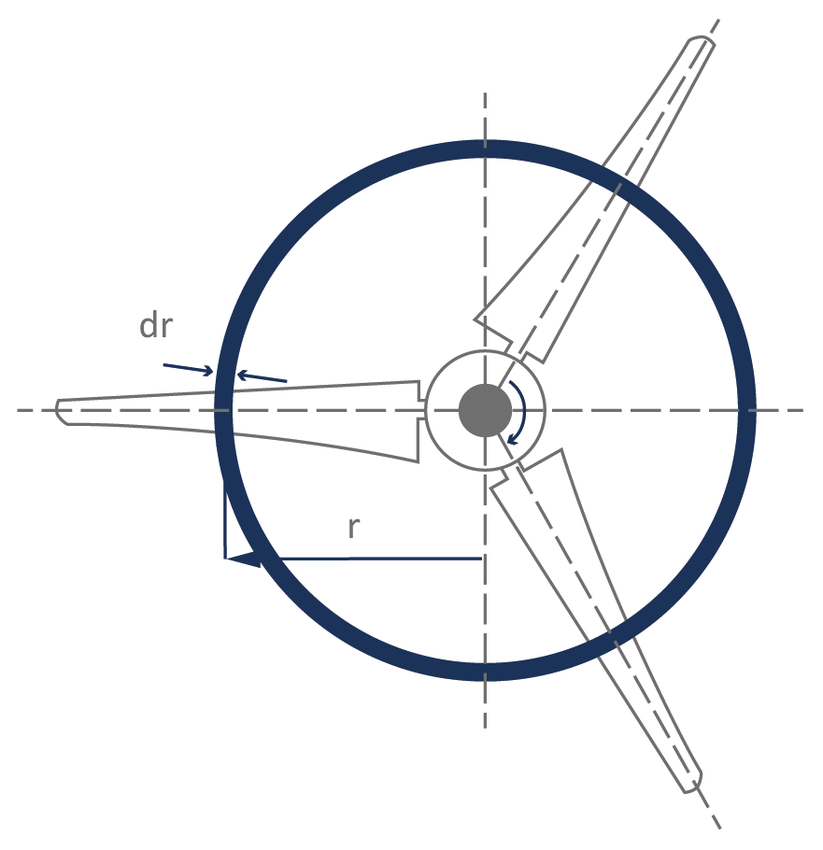
\includegraphics[width=0.8\textwidth]{figures/ringschnitt_rotor.png}
\caption{Schematische Darstellung des Rotorabschnitts für die BEM-Simulation \cite{noauthor_aerodynamik_nodate}}
\label{fig:ringschnitt}
\end{figure}

\section{Besonderheiten sehr kleiner Windkraftanlagen}